\section{Introduction}
\label{sec:introduction}
Despite the outstanding performance Large Language Models (LLMs) exhibit in various tasks~\citep{DBLP:journals/corr/abs-2303-18223, DBLP:journals/corr/abs-2306-02781,DBLP:journals/corr/abs-2406-13035, DBLP:journals/corr/abs-2409-09808, wan2025meda}, the significant resources consumed limit their widespread accessibility~\citep{DBLP:journals/tmlr/Wan0LA0LQYZZC024, DBLP:journals/internet/WangWHZAZK24,zhou2024survey}. Model compression~\citep{DBLP:journals/corr/abs-2308-07633, shen2025efficient} is one effective approach to reduce resource consumption. To avoid resource-intensive retraining, LLM compression is often conducted in a post-training manner. Techniques such as LLM quantization~\citep{DBLP:conf/iclr/YuanSD24, DBLP:conf/icml/HuangLQLZ0M024}, unstructured pruning~\citep{DBLP:conf/icml/FrantarA23}, and structured pruning~\citep{DBLP:conf/nips/MaFW23, DBLP:conf/iclr/AshkboosCNHH24, DBLP:journals/corr/abs-2406-10594} have been proposed.

\begin{figure}[t]
\centering
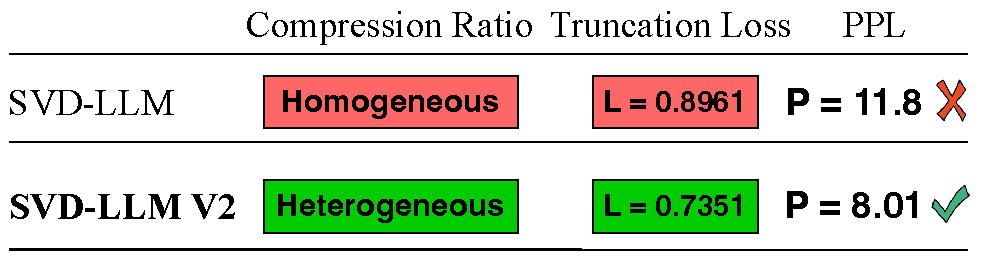
\includegraphics[width=0.48\textwidth]{Figures/Motivation.pdf}
\caption{Comparison between \sysname and SVD-LLM. We randomly select a weight matrix from LLaMA-3 8B and compare the normalized truncation loss and perplexity (PPL) under 20\% compression ratio. }
\label{fig:motivation}
\end{figure}

Low-rank approximation, such as Singular Value Decomposition (SVD) is also an effective technique for compressing LLMs. Compared with quantization and unstructured pruning, SVD compression is more hardware-friendly. 
%
Recently, a few SVD-based LLM compression methods
% such as FWSVD~\citep{DBLP:conf/iclr/HsuHCLSJ22}, ASVD~\citep{DBLP:journals/corr/abs-2312-05821} and SVD-LLM~\citep{DBLP:journals/corr/abs-2403-07378} 
have been proposed. At a high level, these methods all focus on reducing the truncation loss during SVD compression to reserve accuracy.  
%
Specifically, FWSVD~\citep{DBLP:conf/iclr/HsuHCLSJ22} reduces truncation loss by estimating weight importance and preserving more important weights.
%
ASVD~\citep{DBLP:journals/corr/abs-2312-05821} injects a scaling matrix to reduce the truncation loss but was not able to achieve theoretical minimum truncation loss at each LLM layer. 
%
SVD-LLM~\citep{DBLP:journals/corr/abs-2403-07378}, on the other hand, fills this gap by proposing a whitening matrix that obtains theoretical minimum truncation loss at each LLM layer, demonstrating superior performance.  


% However, these methods often exhibit severe performance degradation.
%However, due to XXX, SVD-LLM fails to obtain the theoretical minimum truncation loss in practice. 
%
Despite such advantage, SVD-LLM has two limitations.
%
First, SVD-LLM applies a homogeneous compression ratio to all the weight matrices. This coarse-grained setup unfortunately overlooks the heterogeneity of weight redundancy across different LLM layers. 
%
Second, SVD-LLM utilizes Cholesky decomposition for weight truncation. However, Cholesky decomposition requires the matrix being decomposed to be positive-definite, a condition that is challenging to fulfill in practice. Moreover, Cholesky decomposition introduces numerical instability throughout its iterative process. 
%
As a consequence, SVD-LLM
could still lead to high truncation loss in practice.
%, even under a low compression ratio\footnote{The compression ratio refers to the percentage of model parameters reduced through compression.}. 
%As a result, given the input activation, the output between the compressed weight matrices and the original ones in the LLM will be significantly different, making the compressed LLM behave much poorer than the original LLM. 
%

% \newpage
In this paper, we propose \sysname, a SVD-based post-training LLM compression method that effectively addresses the two limitations of SVD-LLM.
%
First, to address the heterogeneity of weight redundancy across layers, \sysname uses the theoretical truncation loss of
weight matrices at each layer as the guidance to assign a unique compression
ratio to each weight matrix based on its type at different layers.
%allocates compression ratios among the weight matrices in different layers.
%to remove the necessity for the decomposed matrix to be positive-definite and to enhance numerical stability,
Second, \sysname substitutes the Cholesky decomposition with two rounds of SVD for weight truncation, which we prove to achieve the theoretical minimum truncation under the optimized compression ratio.
%
In doing so, \sysname is able to achieve better perplexity with lower truncation loss than SVD-LLM (\cref{fig:motivation}).

%For a better demonstration, we compare the truncation loss and the final performance of SVD-LLM~\citep{DBLP:journals/corr/abs-2403-07378} and \sysname on LLaMA-3 8B. As shown in~\cref{fig:motivation}, \sysname achieves a better perplexity with lower truncation loss than SVD-LLM.

We evaluate \sysname on ten datasets covering various language modeling, classification, and generation tasks as well as five LLMs with various backbones and scales. Our results demonstrate the superiority of \sysname with three key findings:


\vspace{-2mm}
\begin{itemize}
    \item \sysname consistently outperforms state-of-the-art SVD-based LLM compression methods across all ten datasets and five LLMs.
    %, achieving over 99\% lower perplexity under 40\% compression ratios and above.
    \vspace{-2mm}
    \item  \sysname outperforms state-of-the-art structured pruning-based LLM compression methods with up to 28\% lower perplexity under 7 GB memory budget. 
    %
    When comparing to state-of-the-art 1-bit quantization-based LLM compression methods, \sysname outperforms PB-LLM and achieves 5\% lower perplexity. 
    %compressing a 16-bit LLM, \sysname achieves performance comparable to using 1-bit post-training quantization techniques under the same memory budget. 
    %
    Moreover, by combining with 2-bit quantization, \sysname is able to outperform 1-bit BiLLM, demonstrating the promise of combining SVD and quantization-based methods for advancing the frontier of post-training LLM compression.
    %when compressing a 2-bit LLM, \sysname surpasses the performance of the state-of-the-art 1-bit quantization with up to 69\% lower perplexity.
    \vspace{-2mm}
    \item LLMs compressed by \sysname achieve inference speedup on real hardware. In particular, LLMs compressed by \sysname are able to achieve a throughput speedup of up to 2.71$\times$ compared to the original LLMs on a single NVIDIA A100 GPU.
\end{itemize}
